\documentclass[12pt,a4paper]{article}
\usepackage[utf8]{inputenc}
\usepackage[T1]{fontenc}
\usepackage[croatian]{babel}
\usepackage{geometry}
\usepackage{graphicx}
\usepackage{setspace}
\usepackage{titlesec}
\usepackage{caption}
\usepackage{tabularx}
\usepackage{tikz}
\usepackage{pgfplots}
\pgfplotsset{compat=1.18}

\geometry{left=3cm,right=2.5cm,top=2.5cm,bottom=2.5cm}
\onehalfspacing

\titleformat{\section}{\normalfont\Large\bfseries\uppercase}{}{0pt}{}
\titleformat{\subsection}{\normalfont\large\bfseries}{}{0pt}{}

\renewcommand{\contentsname}{SADRŽAJ}
\renewcommand{\listfigurename}{POPIS SLIKA}
\renewcommand{\listtablename}{POPIS TABLICA}

\begin{document}

\begin{titlepage}
    \centering
    {\large SVEUČILIŠTE U ZAGREBU\\}
    {\large FAKULTET STROJARSTVA I BRODOGRADNJE\\}
    \vspace{2.5cm}
    {\Large MEHATRONIČKI SUSTAVI\\}
    \vspace{0.5cm}
    {\Large SEMINAR\\}
    \vspace{1.5cm}
    {\Huge \textbf{ANALIZA ROBUSTNOG UPRAVLJANJA}\\}
    \vspace{1.5cm}
    {\large Ivan Horvat\\}
    \vfill
    {\large Profesor: prof. dr. sc. Pero Perić\\}
    \vspace{1cm}
    {\large Zagreb, 2026.}
\end{titlepage}

\pagenumbering{roman}
\tableofcontents
\newpage
\listoffigures
\newpage
\listoftables
\newpage
\pagenumbering{arabic}

\section{Uvod}
Cilj ovog seminara je analizirati primjenu metoda robustnog upravljanja u suvremenim industrijskim postrojenjima.

\section{2. Poglavlje: Teorijska osnova}
Robustno upravljanje fokusira se na održavanje stabilnosti usprkos parametrarskim neizvjesnostima.

\subsection{2.1. Model neizvjesnosti}
U modelu se razmatraju aditivne i multiplikativne neizvjesnosti.

\subsection{2.2. Sinteza regulatora}
Sinteza se provodi pomoću $H_\infty$ normi.

Slika \ref{fig:blok} prikazuje standardni problem upravljanja.
\begin{figure}[h]
    \centering
    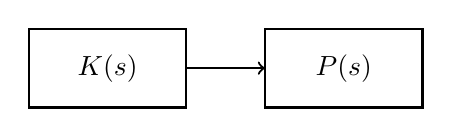
\begin{tikzpicture}
        \draw[thick] (0,0) rectangle (2,1) node[pos=.5] {$K(s)$};
        \draw[thick] (3,0) rectangle (5,1) node[pos=.5] {$P(s)$};
        \draw[->, thick] (2,0.5) -- (3,0.5);
    \end{tikzpicture}
    \caption{Zatvorena upravljačka petlja}
    \label{fig:blok}
\end{figure}

Tablica \ref{tab:usporedba} uspoređuje metode.
\begin{table}[h]
    \centering
    \caption{Usporedba performansi}
    \label{tab:usporedba}
    \begin{tabular}{|c|c|c|}
        \hline
        \textbf{Metoda} & \textbf{Vrijeme smirenja (s)} & \textbf{Preskok (\%)} \\ \hline
        PID & 2.5 & 15 \\ \hline
        $H_\infty$ & 1.8 & 2 \\ \hline
    \end{tabular}
\end{table}

\subsection{2.3. Simulacijski rezultati}
Prikazana je osjetljivost sustava u frekvencijskoj domeni.
\begin{figure}[h]
    \centering
    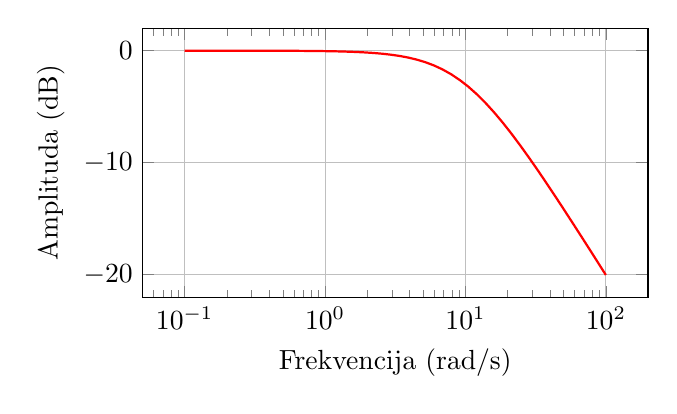
\begin{tikzpicture}
    \begin{axis}[
        width=8cm, height=5cm,
        xmode=log,
        xlabel={Frekvencija (rad/s)},
        ylabel={Amplituda (dB)},
        grid=major
    ]
    \addplot[red, thick, domain=0.1:100, samples=50] {20*log10(1/sqrt(1+(x/10)^2))};
    \end{axis}
    \end{tikzpicture}
    \caption{Bodeov dijagram osjetljivosti}
\end{figure}

\subsection{2.4. Implementacija u realnom vremenu}
Algoritmi su testirani na industrijskom kontroleru.

\section{Zaključak}
Metode pokazuju znatno bolje rezultate u prisutnosti poremećaja u odnosu na klasične pristupe.

\end{document}
